\newpage
	\section{D} \label{sec:D}
	
		\subsection{DEMONSTRABLE}	\index{Demonstrable}	\label{demonstrable}
		Essere in grado di convincere che la scelta fatta è buona. Vengono inoltre prese le decisioni sulle principali interfacce e configurazioni. Ha  a che vedere con la \underline{\hyperref[technologybaseline]{Technology Baseline}}.
	
		\subsection{DIAGRAMMA DI GANTT} \index{Diagramma di Gantt} \label{gantt}
		Il diagramma mostra la dislocazione temporale delle attività per rappresentarne la durata, la sequenzialità, il parallelismo, e confrontarne le stime con i progressi.
		
		\begin{figure}[H]
			\centering
			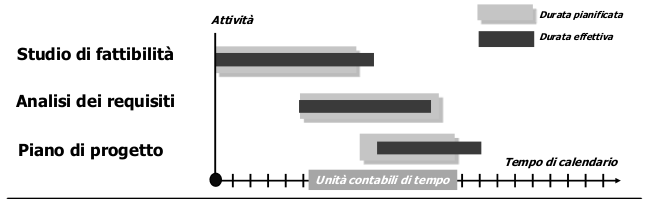
\includegraphics[width=0.5\textwidth]{img/gantt}		
			\caption{Esempio di diagramma di Gantt.}
		\end{figure} 
	
		\subsection{DIAGRAMMA DI PERT} \index{Diagramma di PERT} \label{pert}
		Questo tipo di diagramma (\textit{Programme Evaluation and Review Technique}) mostra le dipendenze temporali tra le varie attività al fine di ragionare sulle scadenze di progetto.
		
		\begin{figure}[H]
			\centering
			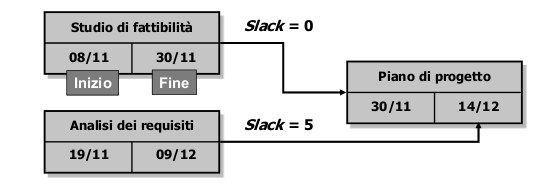
\includegraphics[width=0.5\textwidth]{img/pert}		
			\caption{Esempio di diagramma di PERT.}
		\end{figure} 
		
		Si parla qui di \textit{Slack time}: Si definisce "slack time" il periodo di tempo durante il quale un'attività può essere ritardata senza ritardare l'intero progetto di cui fa parte. Si calcola facendo la differenza tra l'ultima data disponibile per compiere l'attività e la prima data disponibile perché venga compiuta. Il cammino critico è la sequenza di attività ordinata con prodotto importante e dipendenze temporale strette.
		
		\subsection{DIMINISHING RETURNS}	\index{Diminishing returns}	\label{diminishingreturn}	%slide 7/34
		\textit{Ritorno in diminuzione}, c'è un certo punto in cui la curva dell'output decresce, ovvero andare avanti costa di più del beneficio che se ne trae. \\
		È il punto in cui i test non rilevano più gli errori.
		
		\subsection{DIVIDE ET IMPERA}	\index{Divide et Impera} \label{divideetimpera}		
		Se ho un prodotto fatto di parti riesco ad avere parallelismo nell'implementazione, in modo da andare \textit{n} volte più veloce.
		
		\subsection{DOCUMENTI}	\index{Documenti}	\label{documenti}
		I documenti adottano una strategia: come mi approccio al problema e come mitigo i rischi. La milestone è definita dalla strategia e applica il divide-et-impera (perchè divide tutto in problemi più piccoli). La strategia va SEMPRE FATTA ALL'INDIETRO. \\
		Tra i documenti da consegnare alla RR troviamo:
		\begin{itemize}
			\item \underline{\hyperref[piano]{Piano di Progetto}}: quale strategia utilizzare, come nel tempo prepararci ad addomesticare i rischi, ecc;
			\item \underline{\hyperref[norme]{Norme di progetto}};
			\item \underline{\hyperref[pianoqualifica]{Piano di Qualifica}};
			\item \underline{\hyperref[studiofattibilita]{Studio di Fattibilità}};
			\item \underline{\hyperref[analisideirequisiti]{Analisi dei Requisiti}};
		\end{itemize} 
	
		\subsection{DRIVER}	\index{Driver}	\label{driver}
		È una componente attiva fittizia per pilotare il test e serve per eseguire su un'unità che non ha main.
	
